% Source for docs/static/img/marlhf-training.svg. Rebuild from the repository root:
%   pdflatex -output-directory=/tmp docs/scripts/marlhf-training.tex
%   pdf2svg /tmp/marlhf-training.pdf docs/static/img/marlhf-training.svg
%   python3 docs/scripts/prepare_rollout_svgs.py
% Keep the stage boundaries in prepare_rollout_svgs.py in sync with the row positions.
% Shared preamble for the CoMLRL training-flow diagrams. Paste it verbatim at the
% top of every diagram so each .tex stays standalone.
\documentclass[tikz,border=3pt]{standalone}
\usepackage{amsmath,amssymb,bm}
\usetikzlibrary{arrows.meta,positioning,calc,fit}

% Only these paints have dark-theme mappings (assets/_diagram-theme.scss).
\colorlet{agentA}{red!80!black}     % agent 1: policy, prompts, responses, loss
\colorlet{agentB}{blue!80!black}    % agent 2
\colorlet{learned}{orange!80!black} % learned evaluators: critic, reward model
\colorlet{update}{green!50!black}   % gradients and parameter updates
% Joint or shared quantities are black. Gray = black with fill opacity.

\tikzset{
  >={Stealth[length=3.2pt,width=3pt]},
  box/.style={draw, line width=1pt, inner sep=2.5pt, minimum height=13pt},
  policy/.style={box, rounded corners=3pt, minimum width=30pt},
  flow/.style={->, line width=.8pt},
  note/.style={font=\scriptsize, align=left},
  label/.style={anchor=west, font=\footnotesize},
}

% MARLHF: task-reward preference pairs, Stage 1 fits the joint reward model,
% Stage 2 trains the policies with RL on its frozen scores.
% Rows are animation stages; avoid \frac and \_ (their rules animate as edges).
% Rows 0-2 match madpo-training.tex exactly.
\begin{document}
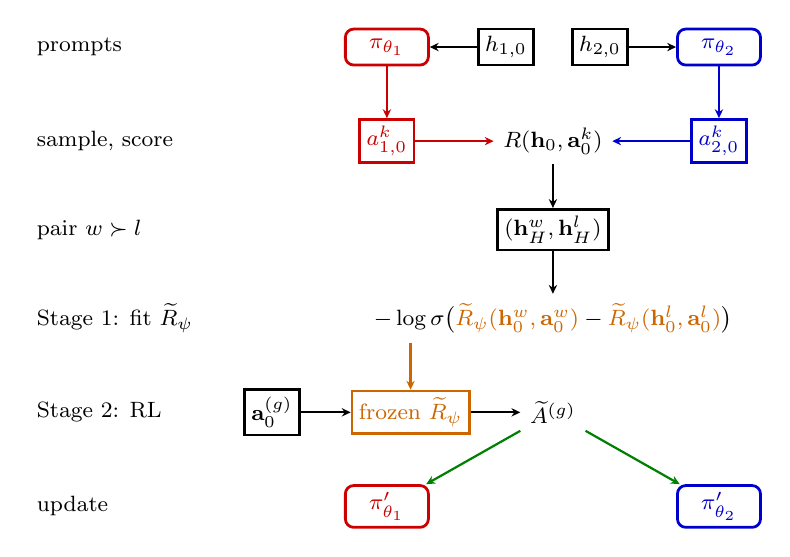
\begin{tikzpicture}[x=1pt, y=1pt, font=\footnotesize]
  \def\xa{130}  % agent 1 column
  \def\xc{190}  % shared column
  \def\xb{250}  % agent 2 column

  % Stage 0: prompts and policies.
  \node[label] at (0,0) {prompts};
  \node[policy, agentA] (p1) at (\xa,0) {$\pi_{\theta_1}$};
  \node[policy, agentB] (p2) at (\xb,0) {$\pi_{\theta_2}$};
  \node[box] (h1) at (\xc-17,0) {$h_{1,0}$};
  \node[box] (h2) at (\xc+17,0) {$h_{2,0}$};
  \draw[flow] (h1) -- (p1);
  \draw[flow] (h2) -- (p2);

  % Stage 1: candidates with the same index k form a joint response and share
  % one task reward.
  \node[label] at (0,-34) {sample, score};
  \node[box, agentA] (a1) at (\xa,-34) {$a^k_{1,0}$};
  \node[box, agentB] (a2) at (\xb,-34) {$a^k_{2,0}$};
  \node (r) at (\xc,-34) {$R(\mathbf{h}_0,\mathbf{a}^k_0)$};
  \draw[flow, agentA] (p1) -- (a1);
  \draw[flow, agentB] (p2) -- (a2);
  \draw[flow, agentA] (a1) -- (r);
  \draw[flow, agentB] (a2) -- (r);

  % Stage 2: a higher-reward joint response is the winner.
  \node[label] at (0,-66) {pair $w\succ l$};
  \node[box] (B) at (\xc,-66) {$(\mathbf{h}^w_H,\mathbf{h}^l_H)$};
  \draw[flow] (r) -- (B);

  % Stage 3: Stage 1, Bradley-Terry fit of the joint reward model.
  \node[label] at (0,-98) {Stage 1: fit $\widetilde{R}_{\psi}$};
  \node (bt) at (\xc,-98) {$-\log\sigma\big(\textcolor{learned}{\widetilde{R}_{\psi}(\mathbf{h}^w_0,\mathbf{a}^w_0)}-\textcolor{learned}{\widetilde{R}_{\psi}(\mathbf{h}^l_0,\mathbf{a}^l_0)}\big)$};
  \draw[flow] (B) -- (bt);

  % Stage 4: Stage 2, the frozen reward model scores new joint responses.
  \node[label] at (0,-132) {Stage 2: RL};
  \node (adv) at (\xc,-132) {$\widetilde{A}^{(g)}$};
  \node[box, learned, anchor=east] (rm) at ([xshift=-18pt]adv.west) {frozen $\widetilde{R}_{\psi}$};
  \node[box, anchor=east] (g) at ([xshift=-18pt]rm.west) {$\mathbf{a}^{(g)}_0$};
  \draw[flow, learned] (rm.north |- bt.south) -- (rm.north);
  \draw[flow] (g) -- (rm);
  \draw[flow] (rm) -- (adv);

  % Stage 5: each agent updates on its own log-probabilities.
  \node[label] at (0,-166) {update};
  \node[policy, agentA] (q1) at (\xa,-166) {$\pi_{\theta_1}'$};
  \node[policy, agentB] (q2) at (\xb,-166) {$\pi_{\theta_2}'$};
  \draw[flow, update] (adv) -- (q1);
  \draw[flow, update] (adv) -- (q2);
\end{tikzpicture}
\end{document}
